\section{Signalbeschreibung \skript{1}}
	\renewcommand{\arraystretchOriginal}{1}
	
	\subsection{Signalklassen \skript{2}}
	
	\begin{minipage}[t]{0.37\textwidth}
		\begin{tabular}{|l|c|l|}
		\hline 
		periodisch & $\Longleftrightarrow$ & nicht-periodisch \\ 
		\hline 
		kontinuierlich & $\Longleftrightarrow$ & zeitdiskret \\ 
		\hline 
		analog & $\Longleftrightarrow$ & digital \\ 
		\hline 
		reell & $\Longleftrightarrow$ & komplex \\ 
		\hline 
		eindimensional & $\Longleftrightarrow$ & mehrdimensional \\ 
		\hline 
		deterministisch & $\Longleftrightarrow$ & stochastisch \\ 
		\hline 
		\end{tabular}
	\end{minipage}
	\begin{minipage}[t]{0.2\textwidth}
		\begin{tabular}{|l|l|}
			\hline \multirow{2}{*}{Nachrichtensignal:}&-Trägt Information\\
			 &-nicht deterministisch\\
			 \hline 
			 \multirow{2}{*}{Hilfssignal:}&-Für das Funktionieren eines Übertragungssystem\\
		 	&-meist periodisch\\
		 	\hline
		 	\multirow{2}{*}{Störsignal:}&-Beeinträchtigt Information (unerwünscht)\\
	 		&-deterministisch oder stochastisch (z.B. Rauschen)\\
 			\hline
		\end{tabular}
	\end{minipage}

	\textbf{Stochastische Signale} sind schwach stationär (Linearer Mittelwert ${X_0}$ und Autokorrelation${\phi_xx}$(t) hängen nicht
	von der Zeit t ab) und können nur durch \textbf{Wahrscheinlichkeitsverteilungen} beschrieben werden.
		\subsubsection{Energie- und Leistungssignale \skript{3}}
		
			\begin{tabularx}{\textwidth}{|p{3.1cm}|c|c|c|}
			\hline
				{}
			&	\multirow{2}{*}{Klasse 1: Energiesignale}
			&	\multicolumn{2}{c|}{Klasse 2: Leistungssignale}
			\\ 
				{}
			&	
			&	Klasse 2a: periodisch
			&	Klasse 2b: aperiodisch
			\\ \hline 
				{}
			&	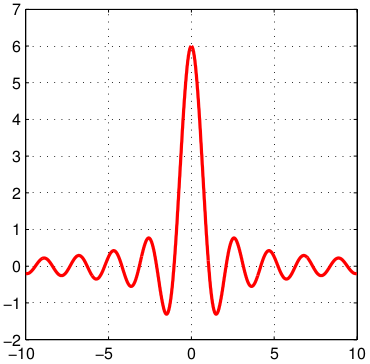
\includegraphics[width=3.3cm]{./bilder/sinc.png}
			& 	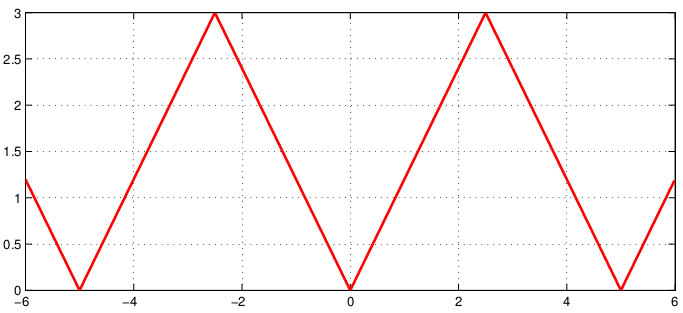
\includegraphics[width=3.5cm]{./bilder/dreieck.png}
			& 	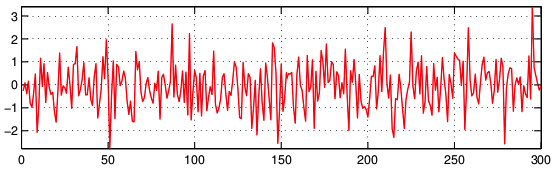
\includegraphics[width=5.29cm]{./bilder/rauschen.png}
			\\ \hline 
				Energie-/Leistungs-dichtesprektrum
			& 	$ E(j \omega) = |F(j \omega)|^2 $
			& 	\multicolumn{2}{c|}{$ \Phi(j\omega) = \lim\limits_{T \to \infty} \dfrac{|F(j\omega)|^2}{T} $}
			\\ \hline 
				Normierte
			& 	$ P_n = 0$
			& 	\formel{$P_n = X^2$} (quadr. Mittelwert)
			& 	$ P_n = \lim\limits_{T \rightarrow \infty} \frac{1}{T} 
									\int\limits_{-T/2}\limits^{T/2} |f(t)|^2 dt $
			\\
				Signalleistung
			&
			& 	(Formeln rechts gelten auch)
			& 	$ P_n = \dfrac{1}{2\pi} \cdot \int\limits_{-\infty}^{\infty} \Phi(j\omega) d\omega $
			\\ \hline
				Normierte
			& 	$ W_n = \lim\limits_{T \rightarrow \infty} \int\limits_{-T/2}\limits^{T/2} |f(t)|^2 dt $
			&	\multicolumn{2}{c|}{$ W_n = \infty $}
			\\
				Signalenergie
			& 	$ W_n = \frac{1}{2 \pi} \int\limits_{-\infty}\limits^{\infty}
									W(j \omega) d\omega $
			&	\multicolumn{2}{c|}{}
			\\ \hline
			\end{tabularx}
				
	\subsection{Mittelwerte \skript{5}}
		
		\begin{tabularx}{\textwidth}{|p{4.7cm}|p{8.1cm}|X|}
			\hline
			Arithmetischer Mittelwert, Linearer MW
		&	$X_0 = \overline{X} = X_m = \frac {1} {T} \int\limits_{-T/2}^{T/2} x(t)dt$
		&	Ist die Fläche unter der Zeitfunktion über eine Periode, nur Klasse 2a
		\\
		\hline
			Quadratischer MW, Leistung
		&	$X^2 = \frac {1} {T} \int\limits_{-T/2}^{T/2} x^2(t)dt$
		& 	nur Klasse 2a
		\\
		\hline
			Mittelwert n. Ordnung
		&	$X^n = \frac {1} {T} \int\limits_{-T/2}^{T/2} x^n(t)dt$
		& 	nur Klasse 2a
		\\
		\hline
			Effektivwert
		&	$X = X_{\text{eff}}= \sqrt{X^2} = \sqrt{\frac{1}{T} \int\limits_{-T/2}^{T/2}{x^2(t)dt}}$
		&	nur Klasse 2a
		\\
		\hline
			Gleichrichtwert
		&	$X_{|m|} = \bar{|X|} = \frac{1}{T} \int\limits_{-T/2}^{T/2}{|x(t)| dt}$
		&	Arithm. Mittelwert der Zweiweggleichrichterschaltung
	    \\
	    \hline
			Varianz
		&	$\text{Var}(x)=\sigma^2= \frac {1} {T} \int\limits_{-T/2}^{T/2}(x(t)-X_0)^2dt = X^2-X_0^2$
		&	Mittlerer Fehler im Quadrat
		\\
		\hline
		Standardabweichung
		&	$\sigma = \sqrt{\text{Var(x)}}$
		&	{}
		\\
		\hline
		\end{tabularx} \\
	
		\textbf{Hinweis:} \\
		\text{\enspace \colorbox{yellow}{Für Signale der \textbf{Klasse 2b} lassen sich Mittelwerte usw. allgemein mit $\lim\limits_{T \rightarrow \infty}$ berechnen!}}\\
		\begin{tabularx}{\textwidth}{llX}
			Für \textbf{reelle Signale} gilt: &
			$ X^2 = |X|^2 = Var(|x|) + |X_0|^2 $ &
			Dies kann die Berechnung des quadratischen Mittelwertes eines zum linearen Mittelwert symmetrischen Signales erleichtern.
		\end{tabularx}
		
		
	\subsection{Autokorrelationsfunktion (AKF) \skript{8}} 
	Die Autokorrelation ist ein Mass für die innere Kohärenz (Ähnlichkeit) eines Signals (Wie weit wird die Zukunft von der Vergangenheit geprägt?).
	
		\bgroup
		\setlength{\tabcolsep}{1mm}
		\begin{tabularx}{\textwidth}{|cX|cX|cX|}
		\hline 
			\multicolumn{2}{|c|}{\textbf{Energiesignale} (Klasse 1)} &
			\multicolumn{2}{|c|}{\textbf{periodische Leistungssignale} (2a)} & 
			\multicolumn{2}{|c|}{\textbf{stochastische Leistungssignale} (2b)}
		\\ \hline 
			$ \varphi_{xx}(\tau) $ &
			$ 		= \lim\limits_{T\to\infty}\int\limits_{-T/2}^{T/2} x(t)x(t-\tau)dt $ \linebreak
				$ 	= \lim\limits_{T\to\infty}\int\limits_{-T/2}^{T/2} x(t+\tau)x(t)dt $ \linebreak
				$	= \varphi_{xx}(-\tau)$ &
			$ \varphi_{xx}(\tau) $ &
			$ 		= \frac {1} {T} \int\limits_{-T/2}^{T/2} x(t)x(t-\tau)dt $ \linebreak
				$	= \frac {1} {T} \int\limits_{-T/2}^{T/2} x(t+\tau)x(t)dt $ \linebreak
				$	= \varphi_{xx}(-\tau) $ &
			$ \varphi_{xx}(\tau) $ &
			$		= \lim\limits_{T\rightarrow\infty} \frac {1} {T} \int\limits_{-T/2}^{T/2} x(t)x(t-\tau)dt $ \linebreak
				$	= \lim\limits_{T\rightarrow\infty}\frac {1} {T} \int\limits_{-T/2}^{T/2} x(t+\tau)x(t)dt $ \linebreak
				$ = \varphi_{xx}(-\tau) $
		\\ \hline
		\end{tabularx} 
		\egroup
		
		\begin{tabularx}{\textwidth}{lX}
		\parbox{6cm}{
			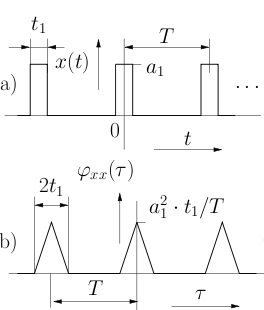
\includegraphics[width=4cm]{./bilder/akf1.png}\\
			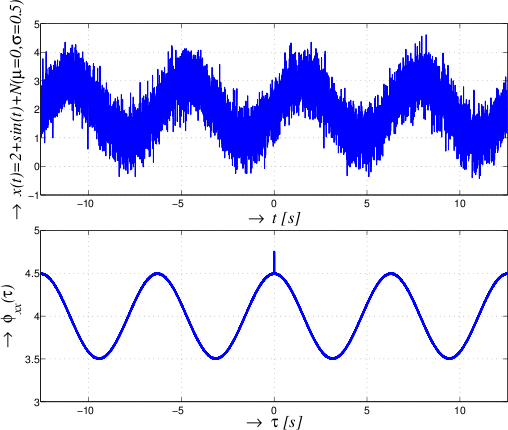
\includegraphics[width=4cm]{./bilder/akf2.png}
		} 
		&
		\parbox{12cm}{
			\textbf{Eigenschaften}
			\begin{itemize}
     			\item $\varphi_{xx}(0) = X^2 = (X_0)^2+\sigma^2$ (Hat immer Diracstoss bei $\tau = 0$)
     			\item $\varphi_{xx}(\tau)=\varphi_{xx}(\tau\pm mT)$, d.h. die AKF
     				ist periodisch mit der gleichen Periode $T$ wie das Signal $x(t)$.
				\item $\varphi_{xx}(\tau)=\varphi_{xx}(-\tau)$: d.h. die AKF ist eine {\bf gerade Funktion}
				\item $\varphi_{xx}(0)\geq|\varphi_{xx}(\tau)|\quad$
				\item $\varphi_{xx}(\tau)\geq (X_0)^2-\sigma^2\quad$
   			\end{itemize}
   			
   			\textbf{Für Leistungssignale gilt:} \ \ \textit{$\Phi(j\omega)$: Leistungsdichtespektrum} \\
   			\fbox{$ \dfrac{1}{2\pi} \cdot \int\limits_{-\infty}^{\infty} \Phi(j\omega) \cdot \e^{j\omega t} d\omega 
						= \colorbox{yellow}{$\varphi_{xx}(t) \ \laplace \ \Phi(j\omega)$} =
						\int\limits_{-\infty}^{\infty} \varphi_{xx}(t) \cdot \e^{-j\omega t} dt $}\\
						
			\textbf{Für Energiesignale gilt:} \ \ \textit{$E(j\omega)$: Energiedichtespektrum} \\
   			\fbox{$ \dfrac{1}{2\pi} \cdot \int\limits_{-\infty}^{\infty} E(j\omega) \cdot \e^{j\omega t} d\omega 
						= \colorbox{yellow}{$\varphi_{xx}(t) \ \laplace \ E(j\omega)$} =
						\int\limits_{-\infty}^{\infty} \varphi_{xx}(t) \cdot \e^{-j\omega t} dt $}\\
   
   			\textbf{Beispiele}
   			\begin{itemize}
     			\item $x(t) = a_k \cos(\omega t + \varphi) \Rightarrow \varphi_{xx}(t) = \frac{a_k^2}{2} \cos(\omega t)$
     			\item $x(t) = b_k \sin(\omega t + \varphi) \Rightarrow \varphi_{xx}(t) = \frac{b_k^2}{2} \cos(\omega t)$
   			\end{itemize}
   		} \\
		\end{tabularx}
				
	\subsection{Kreuzkorrelationsfunktion (KKF) \skript{11}} 
		Die Kreuzkorrelationsfunktion von periodischen Leistungssignalen (Klasse 2a) ist ein Mass für die Ähnlichkeit von zwei verschiedenen Signalen . \textit{''Wie ähnlich sind sich zwei Signale?'' \ \matlab{xcorr}}
		\\	
		\bgroup
		\setlength{\tabcolsep}{1mm}
		\begin{tabularx}{\textwidth}{|cX|cX|cX|}
		\hline 
			\multicolumn{2}{|c|}{\textbf{Energiesignale} (Klasse 1)} &
			\multicolumn{2}{|c|}{\textbf{periodische Leistungssignale} (2a)} & 
			\multicolumn{2}{|c|}{\textbf{stochastische Leistungssignale} (2b)}
		\\ \hline 
			$ \varphi_{xy}(\tau) $ &
			$ 		= \lim\limits_{T\to\infty}\int\limits_{-T/2}^{T/2} x(t)y(t-\tau)dt $ \linebreak
				$ 	= \lim\limits_{T\to\infty}\int\limits_{-T/2}^{T/2} x(t+\tau)y(t)dt $ &
			$ \varphi_{xy}(\tau) $ &
			$ 		= \frac {1} {T} \int\limits_{-T/2}^{T/2} x(t)y(t-\tau)dt $ \linebreak
				$	= \frac {1} {T} \int\limits_{-T/2}^{T/2} x(t+\tau)y(t)dt $ &
			$ \varphi_{xy}(\tau) $ &
			$		= \lim\limits_{T\rightarrow\infty} \frac {1} {T} \int\limits_{-T/2}^{T/2} x(t)y(t-\tau)dt $ \linebreak
				$	= \lim\limits_{T\rightarrow\infty}\frac {1} {T} \int\limits_{-T/2}^{T/2} x(t+\tau)y(t)dt $
		\\ \hline
		\end{tabularx} 
		\egroup

		\begin{tabularx}{\textwidth}{llX}
		\parbox{2.9cm}{
			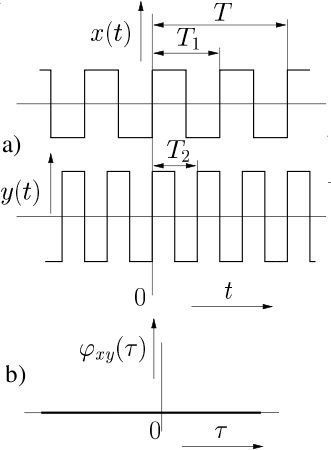
\includegraphics[width=2.9cm]{./bilder/kkf1.png}
		} 
		&
		\parbox{3.9cm}{
			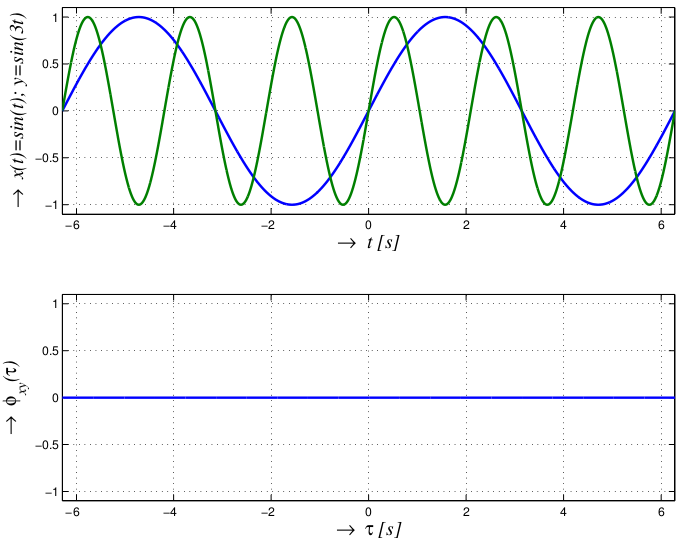
\includegraphics[width=3.9cm]{./bilder/kkf2.png}
		} 
		&
		\parbox{10cm}{
			\textbf{Eigenschaften}
			\begin{itemize}
     			\item Bei Signalen mit verschiedenen Frequenzen ist $\varphi_{xy}$ immer $0$!
     			\item Bei stochastischen Signalen ist $\varphi_{xy}$ immer $0$!
   			\end{itemize}
   			
   			\textbf{Für stochastische Leistungssignale (Klasse 2b) gilt:} \\
   			\fbox{$ \dfrac{1}{2\pi} \int\limits_{-\infty}^{\infty} \Phi_{xy}(j\omega) \e^{j\omega t} d\omega 
						= \colorbox{yellow}{$\varphi_{xy}(t) \ \laplace \ \Phi_{xy}(j\omega)$} =
						\int\limits_{-\infty}^{\infty} \varphi_{xy}(t) \e^{-j\omega t} dt $}\\
   		} \\
		\end{tabularx}
		
		
	\subsection{Rauschen \skript{25} \matlab{randn}}
	
		\begin{tabularx}{\textwidth}{lX}
			\parbox{8cm}{
				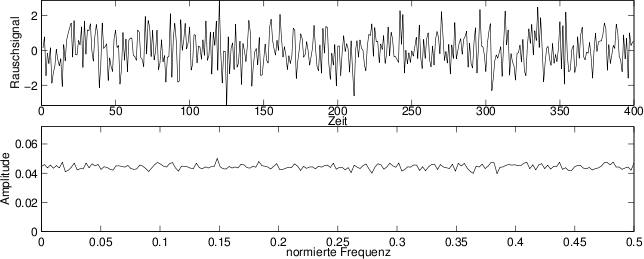
\includegraphics[width=8cm]{./bilder/rauschen2.png}
			} &
			\parbox{9.5cm}{
			Ist die Intensität der
			Rauschspannung "uber viele Frequenzdekaden
			gleich verteilt, so spricht man von \textbf{weissem Rauschen}.\\ \\
			\textbf{Ideale Blindwiderstände verursachen kein Rauschen!}
			\begin{itemize}
     			\item $\text{SNR} = \frac{P_s}{P_r} = \frac{\text{Signalleistung}}{\text{Rauschleistung}}$ (rauschfrei: $ \text{SNR} \rightarrow \infty$) 
     			\item Effektive Rauschspannung: \fbox{$U_r = \sqrt { 4 \cdot k \cdot T \cdot \Delta f \cdot R}$}
     			\item Effektive Rauschleistung: \fbox{$P_r = k \cdot T \cdot \Delta f$}
     			\item Bolzmann-Konstante: $k =1.380662 \cdot 10^{-23}\frac{J}{K}$
   			\end{itemize}
			}
		\end{tabularx}\\
		
	\subsection{Signal-Rausch-Verhältnis (SNR) \skript{27}}
	
		Zur Qualitätsbeurteilung von Signalen wird das Verhältnis zwischen der Leistung des Nutzsignales $P_s$ und der 
		des Rauschsignales $P_r$ gebildet. Dieses Verhältnis wird \textbf{Störabstand} oder \textbf{Rauschabstand} $a_r$ genannt.\\
	
		\begin{minipage}[]{10cm}
			\formel{$a_r = 10 \cdot log_{10} \left(\frac{P_s}{P_r}\right) = 20 \cdot log_{10} \left(\frac{U_s}{U_r}\right)$}
			$[a_r] = dB$\\
		\end{minipage}
		\begin{minipage}[]{10cm}		
			Mindestwert für eine rauschfreie Übertragung: \\
			Musik und Sprache $\rightarrow$ 30 dB \\
			Bilder $\rightarrow$ 40 dB
		\end{minipage}
	
	
	\subsection{Rauschzahl $F$ und Rauschmass $a_F$ \skript{27}}
	
		Jeder Vierpol verkleinert den Rauschabstand des Ausgangssignales gegenüber dem Rauschabstand des Eingangssignales.
		Die Verschlechterung des Rauschleistungsabstandes wird durch die Rauschzahl $F$ \textit{(noise figure)} angegeben.
		Es ist das Verhältnis des Rauschabstandes am Eingang zum Rauschabstand am Ausgang eines Vierpoles.\\
		
		\begin{tabular}{lll}
			\textbf{Rauschzahl:}
		&	\fbox{$F 	= \dfrac{\text{SNR}_{Eingang}}{\text{SNR}_{Ausgang}}
						= \dfrac{\frac{P_{sEingang}}{P_{rEingang}}}{\frac{P_{sAusgang}}{P_{rAusgang}}} 
						= \frac{P_{sEingang}}{P_{rEingang}} \cdot \frac{P_{rAusgang}}{P_{sAusgang}}$}
		&	Idealer Vierpol: $F = 1$
		\\
			\textbf{Rauschmass} (logarithmisch):
		&	\formel{$a_F = 10 \cdot log_{10} (F) = a_{rEingang} - a_{rAusgang}$}
		&	$[a_F] = dB$
		\end{tabular}\\
	
	\subsection{Amplitudenanalyse von Signalen \skript{29}}
	
		\begin{tabular}{ll}
			\parbox{7cm}{
				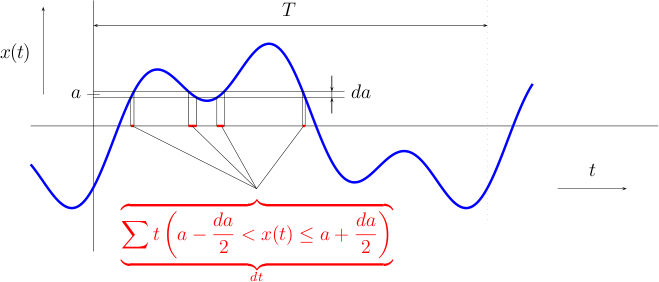
\includegraphics[width=7cm]{./bilder/amplitudenanalyse.png}
			}
		& 	\begin{minipage}[]{11cm}
			Die Amplitudendichte $p(a)$ ist ein Mass für u die relative Zeit ( Zeit / Gesamtzeit =	Wahrscheinlichkeit), während der sich das Signal in einem bestimmten Amplitudenintervall a +- da / 2 aufhält.
			''Zeit während sich Signal in bestimmtem Amplitudenintervall aufhält''\\
				\fbox{$p(a) 	= \lim\limits_{da \rightarrow 0}\frac{\underbrace{\sum t\left(
								a-\frac{da}{2}<x(t)\leq a+\frac{da}{2}\right)}_{dt}}{T\cdot da}
							= \frac{1}{T}\cdot\frac{dt}{da}$}\\
      		\end{minipage}
		\\
			\parbox{7cm}{
				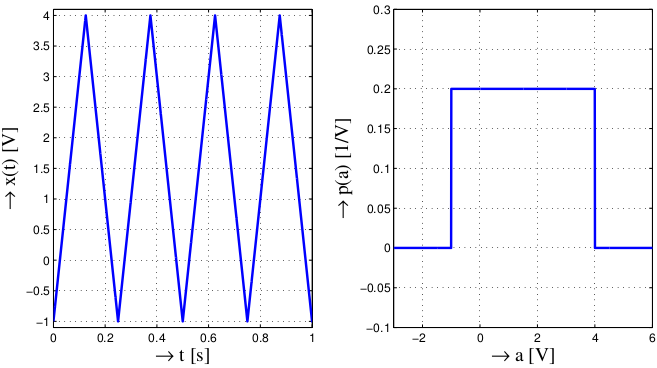
\includegraphics[width=7cm]{./bilder/amplitudenanalyse2.png}
			}
		& 	\begin{minipage}[]{11cm}
				\textbf{Eigenschaften}
				\begin{itemize}
					\item Es gibt keine negativen Werte! $p(a) \geq 0 \ \ \forall a$
     				\item Gesammtwahrscheinlichkeit:\enspace \fbox{$\int\limits_{-\infty}^{\infty} p(a) da = 1$}
     				\item Wahrscheindlichkeit ${a_1 < a < a2}$ \enspace \fbox{$p(a_1 < a < a_2) = \int\limits_{a_1}^{a_2} p(a) da$}
   				\end{itemize}
				
      		\end{minipage}
		\end{tabular}\\ \\
	
		\begin{tabular}{ll}
        		\textbf{Linearer Mittelwert:} \fbox{$X_0  = \int\limits_{-\infty}^{\infty}a\cdot p(a)da$}
        	&	\textbf{Mittelwert $n$. Ordnung:} \fbox{$X^n = \int\limits_{-\infty}^{\infty}a^n\cdot p(a)da$}\\
        	&	\\
        		\textbf{Varianz:} \fbox{$Var(x)  = \int\limits_{-\infty}^{\infty}(a-X_0)^2 \cdot p(a)da$}
        	&
        \end{tabular}\\ \\
	
		\textbf{Beispiel:}\\
		\beispiel{
		\begin{tabularx}{\textwidth}{cX}
			\parbox{7cm}{
				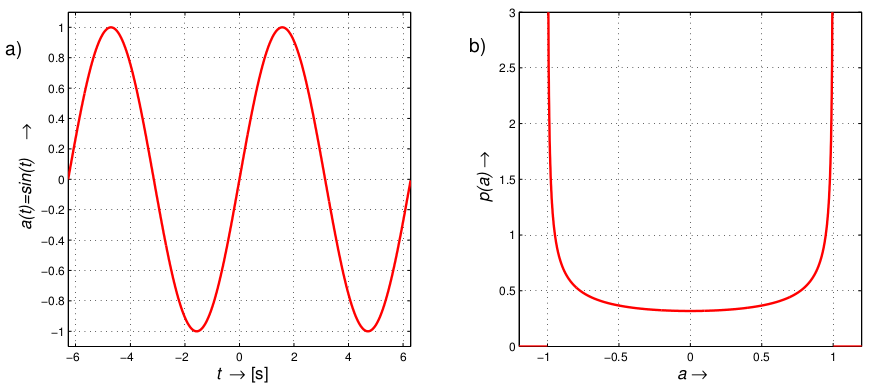
\includegraphics[width=7cm]{./bilder/amplitudenverteilung_bsp1.png}
			}
		&	\begin{minipage}[]{11cm}
				\fbox{$f(t) = sin(t)$} \\
				$t = arcsin(a)$ \\
				$\frac{dt}{da} = 2 \cdot \frac{d(arcsin(a))}{da} = 2 \cdot \frac{1}{\sqrt{1-a^2}}$ \\
				\textit{Der Faktor $2$ kommt daher, dass die Sinusfunktion nicht eindeutig ist!}\\
				\fbox{$p(a) = \frac{1}{T} \cdot \frac{dt}{da} = \frac{2}{2 \pi} \cdot \frac{1}{\sqrt{1-a^2}}$}
      		\end{minipage}
		\end{tabularx}
		}
		
	\subsection{Zentraler Grenzwertsatz}
		\begin{minipage}[]{11cm}
			$X_1, X_2, \ldots , X_n$ sind lauter identisch verteilte (nicht notwendig normalverteilt!)
			unabhängige Zufallsvariablen mit demselben Erwartungswert $\mu$ und derselben Varianz $\sigma^2$
			und mit $Z = \frac{X-\mu}{\sigma}$
		  	Dann hat die Summe
			\begin{equation}
				S_n = \frac{1}{\sqrt{n}}\sum_{i=1}^n Z_i \nonumber
			\end{equation}
			den Erwartungswert $n \mu$ und die Varianz $n \sigma^2$. \\
		  	Die damit verbundene standardisierte ($E(S_n) = 0, var(S_n) = 1$) Variable $S_n$ ist somit wie
		  	folgt definiert: \\ 
			\begin{equation}
				S_n = \frac{1}{\sqrt{n}}\sum_{i=1}^n \frac{X_i - \mu}{\sigma}
				= \frac{1}{\sqrt{n}\cdot \sigma}\left[\left(\sum\limits_{i=1}^n X_i\right) -n \mu\right]
				=\dfrac{\bar{X} - \mu}{\sigma / \sqrt{n}} \nonumber
			\end{equation}
		  	Für $\boldsymbol{n \to \infty}$ strebt die Verteilung von $S_n$ gegen die Standardnormalverteilung. \\
		  \end{minipage}
		  \begin{minipage}[]{8cm}
		  	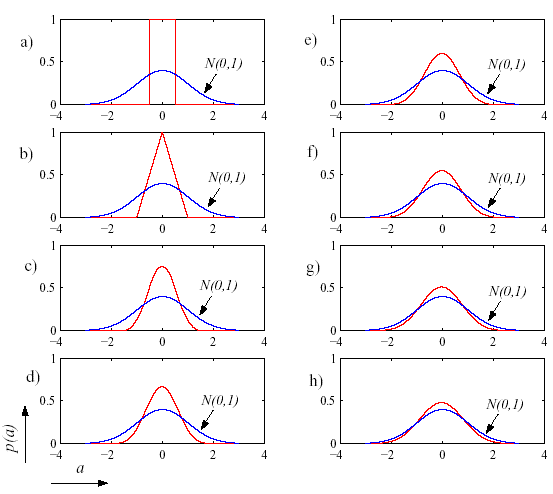
\includegraphics[width=8cm]{./bilder/grenzwertsatz.png}
		  \end{minipage}
	  	
	\subsection{Faltung \skript{34}}
		
		\begin{tabularx}{\textwidth}{lX}
			\parbox{5cm}{
				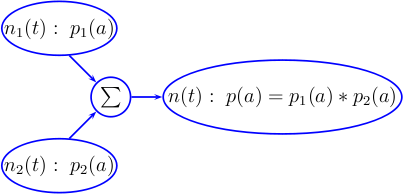
\includegraphics[width=5cm]{./bilder/faltung.png}
			}
			& 	\parbox{13cm}{
				Convolution, ``Addition zweier unabhängiger ergodischer Prozesse $n_i$'' \matlab{conv}\\
				\formel{$p(a) 	= p_1(a) \ast p_2(a)
					= p_2(a) \ast p_1(a)
					= \int\limits_{-\infty}^{\infty}p_1(\xi)\cdot p_2(a-\xi) d\xi$
				} \\
				
				\begin{itemize}
					\item Gesamtbreite der Faltung = Summe der Breiten aller Funktionen
					\item Startpunkt = Summe aller Startpunkte
					\item Endpunkt = Summe aller Endpunkte
					\item $f(t) * g(t) \ \laplace \ F(s) G(s)$
					\item $F(s) * G(s) \ \Laplace \ \frac{1}{2 \pi} f(t) g(t)$
				\end{itemize}
			}
			\\
			\textbf{Faltung zweier Normalverteilungen:}
			&
			Ergibt wieder eine Normalverteilung: \newline
			\fbox{$N(\mu_1, \sigma_1) \ast N(\mu_2, \sigma_2) = 
				N \left( \underbrace{\mu_1 + \mu_2}_{\mu} \underbrace{\sqrt{\sigma_1^2 + \sigma_2^2}}_{\sigma} \right)$}
			\\ & \\
			\textbf{Zentraler Grenzwertsatz:}
			&	Unendlich viele unabhängige Prozesse miteinander gefaltet ergibt
			(unabhängig von den einzelnen Verteilungen) eine \textbf{Normalverteilung}.
		\end{tabularx}
	
	\subsection{Faltung von Grundsignalen}
		\rotatebox{-90}{
			\begin{minipage}[]{22.5cm}
				\begin{tabular}{|c|c|c|c|c|c|}
					\hline
					Kurven
					&	\textbf{Rechtecksimpuls} 
					& 	\textbf{Dreiecksimpuls}
					&	\textbf{Sägezahnimpuls}
					& 	\textbf{Sinuskurve}
					& 	\textbf{E-Kurve}
					\\  % Extra row for graphs
					& & & & & 
					\\ 
					&	%Autor:		Nithuran Selvarajah
%Version:	1.0
%Datum:		21.12.2019

\iffalse
\begin{graphPlot}
	{
		\draw[red, ultra thick, domain=0.01:2] plot (\x, {\x});				% Steigende Gerade
	}
\end{graphPlot}
\fi

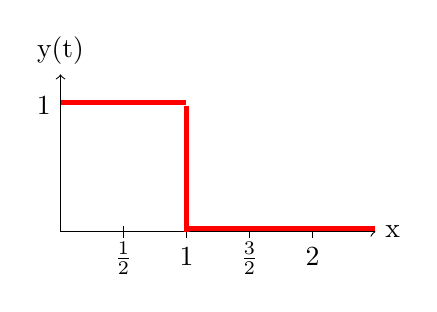
\begin{tikzpicture}[xscale=0.8, yscale=0.8]
	%\draw[help lines] (0,0) grid (6,4);
	\normalsize
	
	\draw [<->] (0, 2.5) -- (0, 0) -- (5, 0);
	\node [right] at (5, 0) {x};				% x-label
	\node [above] at (0, 2.5) {y(t)};			% y-label
	
	\draw (1, -0.1) --  (1, 0.1);				% Strich
	\node [below] at (1, 0) {$\frac{1}{2}$};	% Zahl beim Strich
	\draw (2, -0.1) --  (2, 0.1);
	\node [below] at (2, -0.1) {$1$};
	\draw (3, -0.1) --  (3, 0.1);
	\node [below] at (3, 0) {$\frac{3}{2}$};
	\draw (4, -0.1) --  (4, 0.1);
	\node [below] at (4, -0.1) {$2$};
	
	\node [left] at (0,2) {$1$};
	%\draw [-, red] (0, 3) -- (5, 3);			% Gerade Linie
	\draw[red, ultra thick, domain=0.01:2] plot (\x, {2.05});		% Konstante
	\draw[red, ultra thick] (2, 0) -- (2, 2);						% Senkrechter Strich
	\draw[red, ultra thick, domain=0.01:3] plot (\x + 2, {0.05});	% Konstante

\end{tikzpicture}

					&	%Autor:		Nithuran Selvarajah
%Version:	1.0
%Datum:		21.12.2019

\iffalse
\begin{graphPlot}
	[
	\draw[red, ultra thick, domain=0.01:2] plot (\x + 2, {-(\x - 2)});	% Fallende Gerade
	]
	{
		\draw[red, ultra thick, domain=0.01:2] plot (\x, {\x});				% Steigende Gerade
	}
\end{graphPlot}
\fi

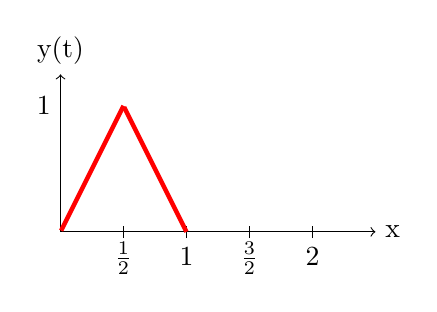
\begin{tikzpicture}[xscale=0.8, yscale=0.8]
	%\draw[help lines] (0,0) grid (6,4);
	\normalsize
	
	\draw [<->] (0, 2.5) -- (0, 0) -- (5, 0);
	\node [right] at (5, 0) {x};				% x-label
	\node [above] at (0, 2.5) {y(t)};			% y-label
	
	\draw (1, -0.1) --  (1, 0.1);				% Strich
	\node [below] at (1, 0) {$\frac{1}{2}$};	% Zahl beim Strich
	\draw (2, -0.1) --  (2, 0.1);
	\node [below] at (2, -0.1) {$1$};
	\draw (3, -0.1) --  (3, 0.1);
	\node [below] at (3, 0) {$\frac{3}{2}$};
	\draw (4, -0.1) --  (4, 0.1);
	\node [below] at (4, -0.1) {$2$};
	
	%\draw [dashed, red] (0, 3) -- (5, 3);		% Gestrichelte Linie
	\node [left] at (0,2) {$1$};
	\draw[red, ultra thick, domain=0.01:1] plot (\x, {2*\x});			% Steigende Gerade (Input, Output)
	\draw[red, ultra thick, domain=0.01:1] plot (\x + 1, {-2*\x + 2});	% Fallende Gerade
\end{tikzpicture}

					&	%Autor:		Nithuran Selvarajah
%Version:	1.0
%Datum:		21.12.2019

\begin{tikzpicture}[xscale=0.8, yscale=0.8]
	%\draw[help lines] (0,0) grid (6,4);
	\normalsize
	
	\draw [<->] (0, 2.5) -- (0, 0) -- (5, 0);
	\node [right] at (5, 0) {x};				% x-label
	\node [above] at (0, 2.5) {y(t)};			% y-label
	
	\draw (1, -0.1) --  (1, 0.1);				% Strich
	\node [below] at (1, 0) {$\frac{1}{2}$};	% Zahl beim Strich
	\draw (2, -0.1) --  (2, 0.1);
	\node [below] at (2, -0.1) {$1$};
	\draw (3, -0.1) --  (3, 0.1);
	\node [below] at (3, 0) {$\frac{3}{2}$};
	\draw (4, -0.1) --  (4, 0.1);
	\node [below] at (4, -0.1) {$2$};
	
	\node [left] at (0,2) {$1$};
	%\draw [-, red] (0, 3) -- (5, 3);			% Gerade Linie
	\draw[red, ultra thick] (0.01, 0.01) -- (0.01, 2);				% Senkrechter Strich
	\draw[red, ultra thick, domain=0.01:1] plot (\x, {-2*\x + 2});	% Fallende Gerade

\end{tikzpicture}
					&	\input{tikz/sinus.tex}
					&	\input{tikz/e_kurve.tex}
					\\  \hline
					\textbf{Rechteckimpuls}
					& & & & & 
					\\ 	% Leave free the first cell of row
					&	%Autor:		Nithuran Selvarajah
%Version:	1.0
%Datum:		23.12.2019

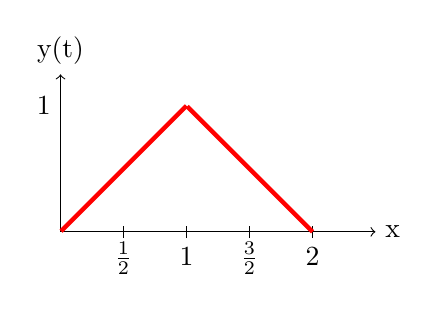
\begin{tikzpicture}[xscale=0.8, yscale=0.8]
	%\draw[help lines] (0,0) grid (6,4);
	\normalsize
	
	\draw [<->] (0, 2.5) -- (0, 0) -- (5, 0);
	\node [right] at (5, 0) {x};				% x-label
	\node [above] at (0, 2.5) {y(t)};			% y-label
	
	\draw (1, -0.1) --  (1, 0.1);				% Strich
	\node [below] at (1, 0) {$\frac{1}{2}$};	% Zahl beim Strich
	\draw (2, -0.1) --  (2, 0.1);
	\node [below] at (2, -0.1) {$1$};
	\draw (3, -0.1) --  (3, 0.1);
	\node [below] at (3, 0) {$\frac{3}{2}$};
	\draw (4, -0.1) --  (4, 0.1);
	\node [below] at (4, -0.1) {$2$};
	
	%\draw [dashed, red] (0, 3) -- (5, 3);		% Gestrichelte Linie
	\node [left] at (0,2) {$1$};
	\draw[red, ultra thick, domain=0.01:2] plot (\x, {\x});				% Steigende Gerade
	\draw[red, ultra thick, domain=0.01:2] plot (\x + 2, {-(\x - 2)});	% Fallende Gerade
\end{tikzpicture}
					&	%Autor:		Nithuran Selvarajah
%Version:	1.0
%Datum:		25.12.2019

\pgfmathdeclarefunction{gauss}{2}{%
	\pgfmathparse{1/(#2*sqrt(2*pi))*exp(-((\x-#1)^2)/(2*#2^2))}	% Gauss curve definition
}

\begin{tikzpicture}[xscale=0.8, yscale=0.8]
	\draw [<->] (0, 2.5) -- (0, 0) -- (5, 0);
	\node [right] at (5, 0) {x};				% x-label
	\node [above] at (0, 2.5) {y(t)};			% y-label
	
	\draw (1, -0.1) --  (1, 0.1);				% Strich
	\node [below] at (1, 0) {$\frac{1}{2}$};	% Zahl beim Strich
	\draw (2, -0.1) --  (2, 0.1);
	\node [below] at (2, -0.1) {$1$};
	\draw (3, -0.1) --  (3, 0.1);
	\node [below] at (3, 0) {$\frac{3}{2}$};
	\draw (4, -0.1) --  (4, 0.1);
	\node [below] at (4, -0.1) {$2$};
	
	\node [left] at (0,2) {$1$};
	
	\draw[red, ultra thick, domain=0:4] plot (\x, {4*gauss(2, 0.75)});	% Gauss
\end{tikzpicture}
					&	%Autor:		Nithuran Selvarajah
%Version:	1.0
%Datum:		25.12.2019

\pgfmathdeclarefunction{gauss}{2}{%
	\pgfmathparse{1/(#2*sqrt(2*pi))*exp(-((\x-#1)^2)/(2*#2^2))}	% Gauss curve definition
}

\begin{tikzpicture}[xscale=0.8, yscale=0.8]
	\draw [<->] (0, 2.5) -- (0, 0) -- (5, 0);
	\node [right] at (5, 0) {x};				% x-label
	\node [above] at (0, 2.5) {y(t)};			% y-label
	
	\draw (1, -0.1) --  (1, 0.1);				% Strich
	\node [below] at (1, 0) {$\frac{1}{2}$};	% Zahl beim Strich
	\draw (2, -0.1) --  (2, 0.1);
	\node [below] at (2, -0.1) {$1$};
	\draw (3, -0.1) --  (3, 0.1);
	\node [below] at (3, 0) {$\frac{3}{2}$};
	\draw (4, -0.1) --  (4, 0.1);
	\node [below] at (4, -0.1) {$2$};
	
	\node [left] at (0,2) {$1$};
	
	\draw[red, ultra thick, domain=2:4] plot (\x - 2, {4*gauss(2, 0.75)});	% Halb-Gauss
\end{tikzpicture}
					&	
					&	
					\\ \hline 
					\textbf{Dreieckimpuls}
					& & & & &
					\\ 
					& 	
					&	
					& 	
					&	
					&	
					\\ \hline  
					\textbf{Sägezahn}
					& & & & & 
					\\ 
					&	
					&
					&	
					&	
					&
					\\ \hline      
					\textbf{Sinuskurve}
					& & & & &
					\\ 
					& 	
					& 
					& 	
					&
					&	
					\\ \hline
					\textbf{E-Kurve}
					& & & & & 
					\\ 
					& 	
					& 	
					& 	
					&	
					&
					\\ \hline
				\end{tabular}\\ \\
			\end{minipage}
		}
	\newpage
	
	\subsection{Stochastische Signale und deren Verteilungen \skript{38}}
		\rotatebox{90}{
		\begin{minipage}[]{22.5cm}
			\begin{tabular}{|c|c|c|c|c|}
			\hline
				Verteilung
			& 	\textbf{gleichverteilt}
			& 	\textbf{gaussförmig}
			& 	\textbf{sinusförmig}
			&	\textbf{exponentiell}
			\\ \hline\hline
			& 	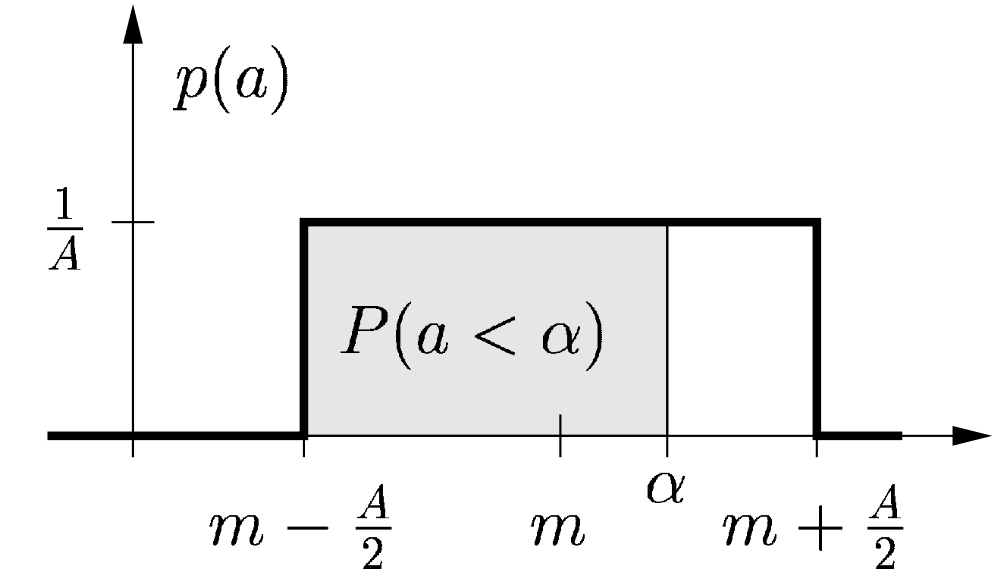
\includegraphics[width=4.3cm]{./bilder/verteilungen-gleichvert.png}
			&	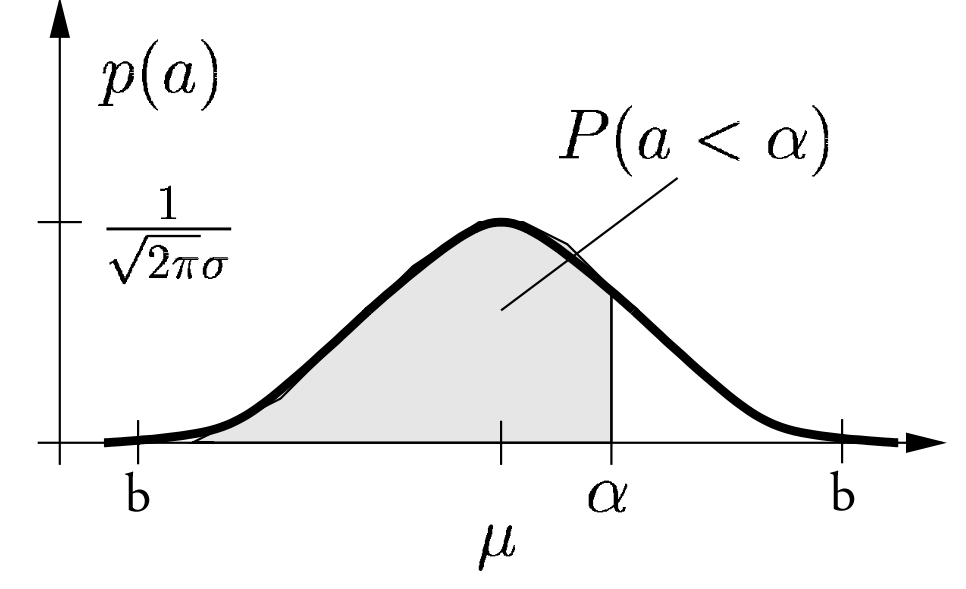
\includegraphics[width=4.3cm]{./bilder/verteilungen-gauss.png}
			&	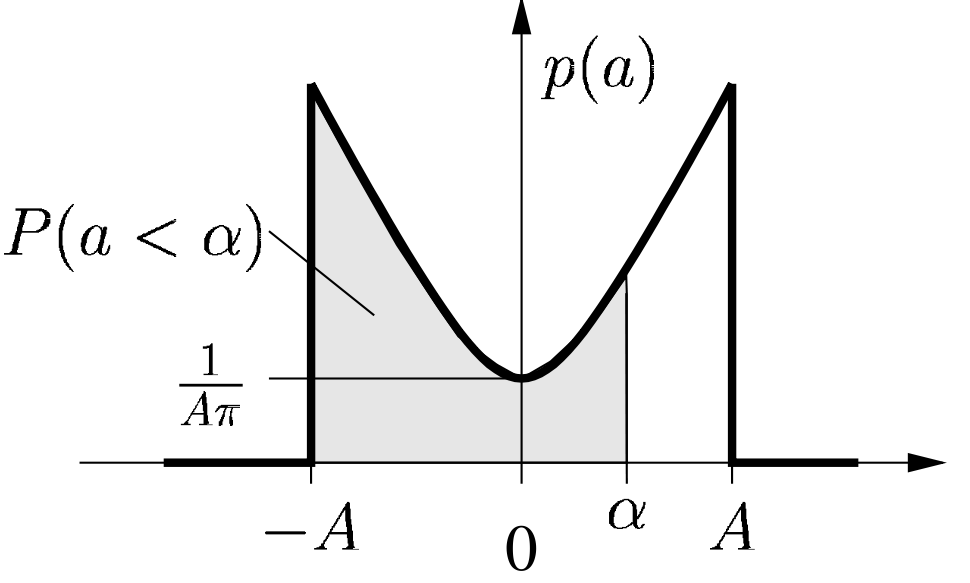
\includegraphics[width=4.3cm]{./bilder/verteilungen-sinus.png}
			&	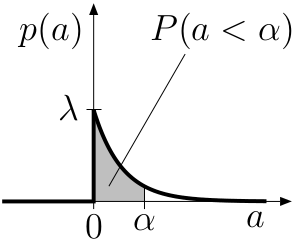
\includegraphics[width=3cm]{./bilder/verteilungen-exp.png}
			\\ \hline 
				Amplitudendichte
			& & & &
			\\ 
				$p(a)=$
			& 	$\begin{cases} \frac{1}{A}&|a-m|\leq \frac{A}{2},\\ 0&|a-m|>\frac{A}{2}.\\ \end{cases}$
			&	$\displaystyle\frac{1}{\sigma \sqrt{2\pi}}e^{\displaystyle\frac{-(a-\mu)^2}{2\sigma^2}}$
			& 	$\begin{cases} \frac{1}{\pi\sqrt{A^2-a^2}}&|a|\leq A,\\ 0&|a|>A.\\ \end{cases}$
			&	$\begin{cases} \lambda \e^{-\lambda a} & a \geq 0, \\ 0 & a<0.\\ \end{cases}$
			\\ \hline  
			 	Wahrscheinlichkeit,
			& & & &
			\\ 
				dass die Amplitude $a$
			& & & &
			\\  
				kleiner gleich $\alpha$ ist
			& & & &
			\\ 
				$P(a\!\leq\!\alpha)\!=\!\!\int\limits_{-\infty}^{\alpha}\!p(a)da=$
			&	$\begin{cases}0&\alpha<m-\frac{A}{2},\\ \frac{\alpha-(m-\frac{A}{2})}{A}&
					|\alpha-m|\leq\frac{A}{2} \\1&\alpha\geq m+\frac{A}{2}. \end{cases}$
			&	$Q\left(\frac{\displaystyle\mu-\alpha}{\displaystyle\sigma}\right)$
			&	$\begin{cases}0&\alpha\!\leq\!-A,\\ \frac{1}{\pi}\left(\frac{\pi}{2}\!+\!\sin^{-1}\!
					\left(\frac{a}{A}\right)\right)&|\alpha|\!<\!A,\\1&\alpha\geq A. \end{cases}$ 
			&	$\begin{cases} 0 & a < 0, \\ 1-\e^{-\lambda a} & a \geq 0.\\ \end{cases}$
			\\ \hline      
			& & & &
			\\ 
				linearer Mittelwert $X_0 =$
			& 	$m$
			& 	$\mu$
			& 	$0$
			&	$\dfrac{1}{\lambda}$
			\\ 
			& & & &
			\\ \hline
			& & & &
			\\
				Varianz $\operatorname{Var}(x) = $
			& 	$\dfrac{A^2}{12}$
			& 	$\sigma^2$ 
			& 	$\dfrac{A^2}{2}$ 
			&	$\dfrac{1}{\lambda^2}$
			\\
				$X^2 - X_0^2$ & & & &
			\\ \hline
			& & & &
			\\
				Leistung $X^2 =$
			& 	$m^2+\dfrac{A^2}{12}$ 
			&	$\mu^2+\sigma^2$ 
			& 	$\dfrac{A^2}{2}$
			&	$\dfrac{2}{\lambda^2}$
			\\
				$\operatorname{Var}(x) + X_0^2$
			& & & &
			\\
				(quadratischer Mittelwert) 
			& & & &
			\\ \hline
			\end{tabular}\\ \\
			\textbf{Anmerkung zur gaussförmigen Verteilung:}\\
			Im Intervall $\mu \pm 3\sigma$ sind 99,73\% aller Messwerte zu finden.
			In der Zeichung ist diese Stelle mit \textbf{b} gekennzeichnet.\\ \\
			Allgemein: \formel{$\operatorname{Var}(x) = X^2 - X_0^2$}
		\end{minipage}
		}
		\newpage

		
		
%	\subsection{Q-Funktion \skript{41}}
%	
%		\begin{tabular}{ll}
%			\parbox{6cm}{
%				Tabelle \skript{52} \\
%				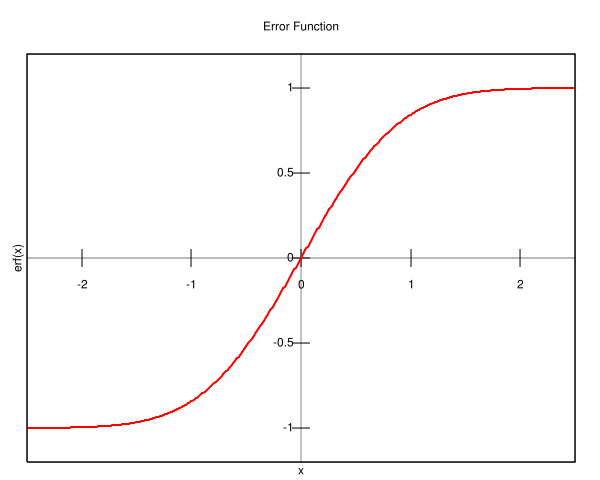
\includegraphics[width=5cm]{./bilder/q-funktion.png}
%			}
%		& 	\parbox{12cm}{
%				``Wahrscheinlichkeit eines Fehlers'' \matlab{erf, erfc} \\
%				Wenn die Resultate einer Messserie mit einer Normalverteilung mit Varianz
%				$\sigma$ und Erwartungswert $0$ auftreten, dann ist
%				$\operatorname{erf}\,\left(\,\frac{a}{\sigma \sqrt{2}}\,\right)$ die
%				Wahrscheinlichkeit, dass ein einzelner Messwert zwischen $-a$ und $a$ liegt. 
%				\\
%				\fbox{$Q(\xi) = 1-Q(-\xi) = \frac{1}{\sqrt{2\pi}}\int\limits_{\xi}^{\infty}
%				e^{-\frac{y^2}{2}}dy$} \\
%				\fbox{$Q(\xi) = \frac12 \operatorname{erfc}\left(\frac{\xi}{\sqrt2}\right)
%				= \frac12 \left(1 - \operatorname{erf}\left( \frac{\xi}{\sqrt2}\right) \right)$} \\
%			}
%		\end{tabular}
%	
%	
%	\subsubsection{Beispiel: Wahrscheinlichkeit einer Falschdetektierung eines Schwellwertdetektors \skript{40}}
%		
%		\begin{tabularx}{\textwidth}{ccX}
%			\multicolumn{2}{c}{
%				\parbox{7cm}{
%					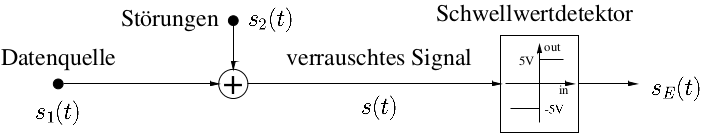
\includegraphics[width=7cm]{./bilder/schwellwertdetektor1.png}
%				}
%			}
%		&	\beispiel{\parbox{10.5cm}{
%				\textbf{Gegeben:} $\mu = 0V$, $\sigma^2 = 1V^2$\\
%				$P_{F1}$ ist die Fehlerwahrscheinlichkeit, dass 5V gesendet wurde, der Detektor sich aber für -5V entschieden hat
%				($P_{F2}$ umgekehrt).
%			}}
%		\\
%			\parbox{2.5cm}{
%				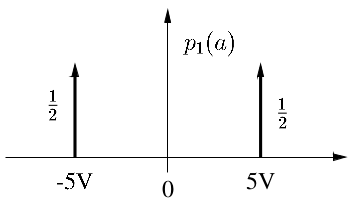
\includegraphics[width=3.5cm]{./bilder/schwellwertdetektor2.png}
%			}
%		&	\parbox{2.5cm}{
%				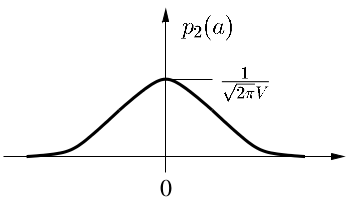
\includegraphics[width=3.5cm]{./bilder/schwellwertdetektor3.png}
%			}
%		& 	\beispiel{\parbox{10.5cm}{
%				$P_{F2} 	= \frac{1}{2} \cdot \int\limits_{0V}^{\infty V} p_2(a+5V) da
%						= \frac{1}{2} \cdot \int\limits_{0V}^{\infty V} \dfrac{1}{1V \cdot \sqrt{2 \pi}} \e^{\dfrac{-(a+5V)^2}{2 \cdot 1V^2}} da $\\
%				$P_{F1} 	= \frac{1}{2} \cdot \int\limits_{-\infty V}^{0V} p_2(a-5V) da
%						= \frac{1}{2} \cdot \int\limits_{-\infty V}^{0V} \dfrac{1}{1V \cdot \sqrt{2 \pi}} \e^{\dfrac{-(a-5V)^2}{2 \cdot 1V^2}} da $
%			}}
%		\\
%			\multicolumn{2}{c}{
%				\parbox{7cm}{
%					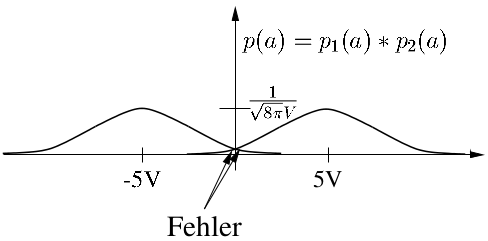
\includegraphics[width=7cm]{./bilder/schwellwertdetektor4.png}
%				}
%			}
%		&	\beispiel{\parbox{10.5cm}{
%				\textbf{Substitution:} $y = \dfrac{a-5V}{1V}$, $dy = \dfrac{da}{1V}$ \\
%				\fbox{$P_{F1} = \frac{1}{2} \cdot \int\limits_{-\infty}^{-5} \dfrac{1}{\sqrt{2 \pi}} \e^{\dfrac{-y^2}{2}} dy 
%						= \frac{1}{2} \cdot \int\limits_{5}^{\infty} \dfrac{1}{\sqrt{2 \pi}} \e^{\dfrac{-y^2}{2}} dy 
%						= \frac{1}{2} \cdot Q(5) $} \\
%				\fbox{$P_{F2} 	= \frac{1}{2} \cdot Q(5) $} \\
%				\textbf{Gesamte Fehlerwahrscheinlichkeit:}\\
%				\fbox{$P_F = P_{F1} + P_{F2} = Q(5) = 2.867 \cdot 10^{-7}$}
%			}}
%		\\ 
%		\end{tabularx}

	\subsection{Zusammenstellung einiger wichtiger Funktionen \skript{44}}
		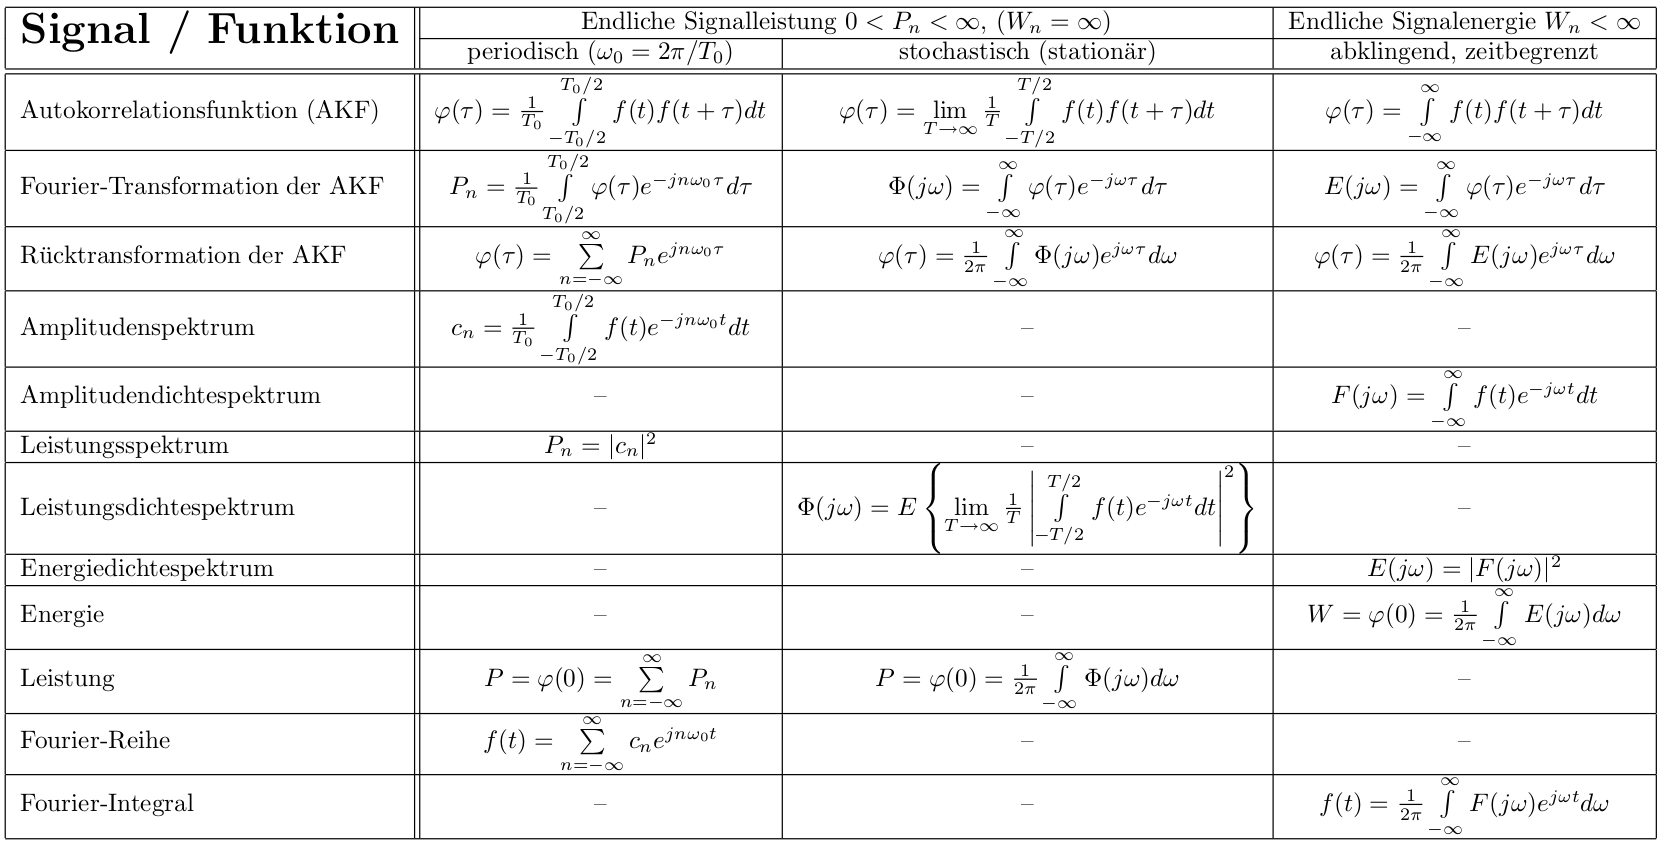
\includegraphics[width=24.5cm,angle=90]{./bilder/zusammenstellung.png}
	